
\newpage
\appendix
\thispagestyle{plain}

\setcounter{figure}{0}
\renewcommand\thefigure{A.\arabic{figure}}

\setcounter{table}{0}
\renewcommand\thetable{A.\arabic{table}}

\section{VCA vs. VCA Competition}
\label{appendix:vca_vs_vca}
We include the following figures to demonstrate that most VCAs can achieve their
nominal uplink utilization rate when in competition with the other VCAs on a 
3 Mbps uplink capacity, the minimum uplink capacity recommended by the FCC (25/3). 
The only exception is two competing Teams calls, which we discuss in Section 5. 
%\FloatBarrier



\begin{figure}[]
\centering
\begin{subfigure}[t]{.4\textwidth}
    \centering
    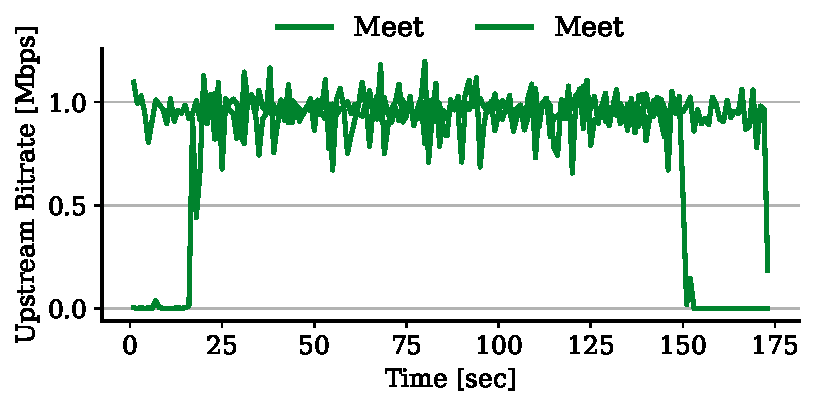
\includegraphics[width=1\textwidth]{figures/appendix/meet_meet_3_ul_r2.pdf}
    \caption{Meet vs. Meet}
    \label{subfig:meet-meet-3}
\end{subfigure}\hfill
\begin{subfigure}[t]{.4\textwidth}
    \centering
    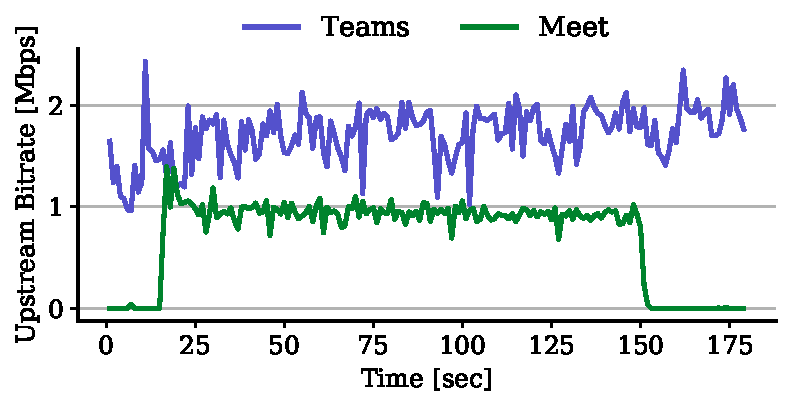
\includegraphics[width=1\textwidth]{figures/appendix/teams_meet_3_ul_r3.pdf}
    \caption{Teams vs. Meet}
    \label{subfig:teams-meet-3}
\end{subfigure}
\begin{subfigure}[t]{.4\textwidth}
    \centering
    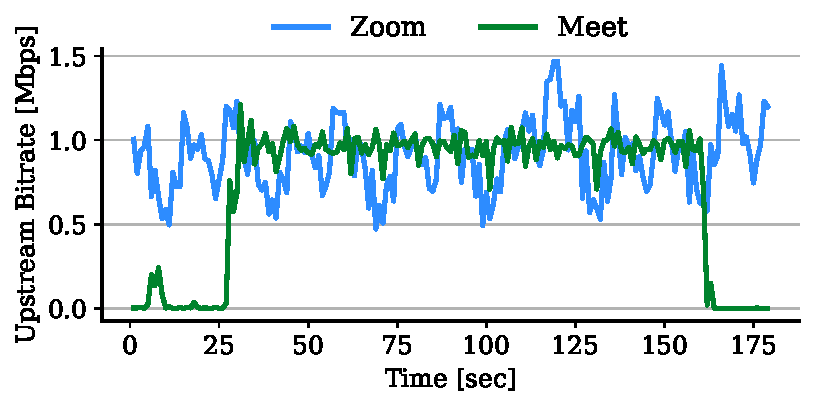
\includegraphics[width=1\textwidth]{figures/appendix/zoom_meet_3_ul_r2.pdf}
    \caption{Zoom vs. Meet}
    \label{subfig:zoom-meet-3}
\end{subfigure}
\begin{subfigure}[t]{.4\textwidth}
    \centering
    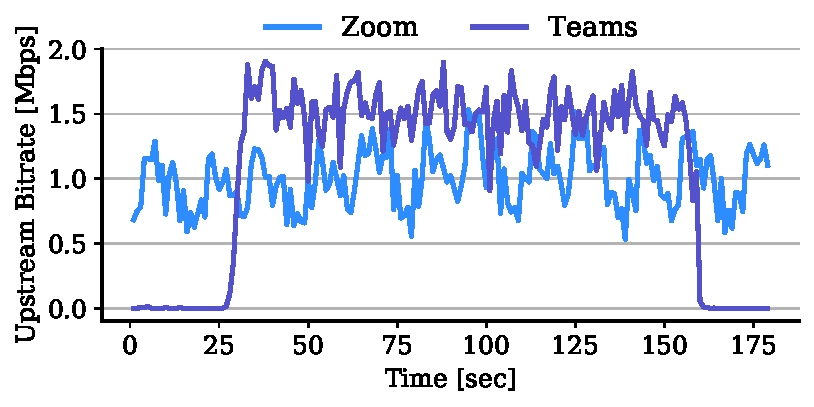
\includegraphics[width=1\textwidth]{figures/appendix/zoom_teams_3_ul_r2.pdf}
    \caption{Zoom vs. Teams}
    \label{subfig:zoom-teams-3}
\end{subfigure}
\begin{subfigure}[t]{.4\textwidth}
    \centering
    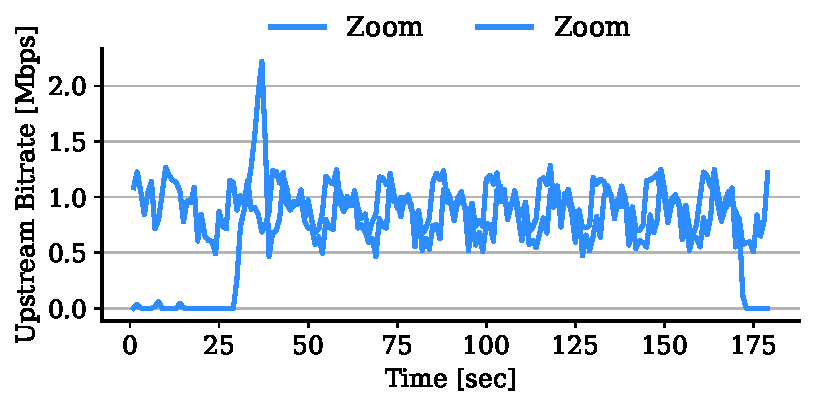
\includegraphics[width=1\textwidth]{figures/appendix/zoom_zoom_3_ul_r1.pdf}
    \caption{Zoom vs. Zoom}
    \label{subfig:zoom-zoom-3}
\end{subfigure}
\caption{VCA vs. VCA on a 3 Mbps symmetric connection.}
\label{fig:vca-vca-3}
\end{figure}

\section{Static Experiments - Repetition on Mac Operating System (MACOS)}
\label{appendix:static}
Here, we demonstrate the extensibility of our automation framework for macOS. More specifically, we repeat the experiments from Section~\ref{sec:static} with the uplink shaped on a device running macOS. We use a 2017 MacBook Air with 8GB 1600 Mhz DDR3 memory, 1.8 GHz Dual-Core Intel Core i5 processor, and Intel HD Graphics 6000 1536 MB Graphics. The laptop is running macOS Version 10.15.7. The MacBook Air initiates a call with a Linux client with the same specifications as outlined in Section 2.2. We use Zoom Version 5.7.6 and Chrome Version 92.0.4515.159. We test the
browser version of Teams and the native client of Zoom and Meet. 

There were also some platform-specific differences while trying to automate the data collection. The macOS does not support v4l2loopback; instead we use Open Broadcaster Software or OBS (Version 27.0.1) to feed in the same
talking-head video used throughout our experiments. In addition, we only include the \teamsbrowser client for Teams and omit the native client. This is because the current version of the Teams client on macOS does not support virtual camera~\cite{teams_virtual_camera}. 


\begin{comment}
\begin{table}[]
\begin{tabular}{|c|c|c|}
\hline
\multirow{2}{*}{\textbf{VCA}} & \multicolumn{2}{c|}{\textbf{Utilization (Mbps)}} \\ \cline{2-3} 
                              & Upstream               & Downstream              \\ \hline
Meet                          & 0.89                   & 0.83                    \\ \hline
Teams                         & -                      & 1.43                    \\ \hline
Zoom                          & 0.96                   & 0.88                    \\ \hline
\end{tabular}
\caption{Unconstrained network utilization on macOS}
\label{tab:vca_static_mac}
\end{table}
\end{comment}

\textbf{Results}: 
Figure~\ref{fig:uplink_static_mac} shows the uplink network utilization on the macOS device with uplink network utilization on Ubuntu shown as a baseline. The overall trends are similar as on Ubuntu. We do find few differences between the two platforms: % Looking first at Figure ~\ref{subfig:vca_static_mac}, the VCAs follow similar trends as in Figure 
%~\ref{subfig:uplink_bitrate},
\zoom has a higher nominal utilization on macOS ($0.96$ Mbps) than Ubuntu ($0.78$ Mbps). \teamsbrowser also has a higher
nominal utilization on macOS than Ubuntu. \meet has a 
similar uplink utilization, using $0.89$ Mbps on Mac and $0.95$ Mbps on Ubuntu. Some of these differences could be due to updated VCA version itself, while others could be attributed to the differences in the operating system. 


We next report application performance metrics (see Figure~\ref{fig:video_qual_comparison}) by logging the WebRTC stats API as in Section~\ref{subsec:application_performance}. The Ubuntu statistics under the same shaping levels are also reported as a baseline. We find that \meet adapts to the constrained throughput setting mainly by increasing the quantization parameter. On the other hand, \teamsbrowser simultaneously adapts both the sent frames per second and the quantization parameter of the encoded video. Interestingly, there are some minor differences compared to Ubuntu. For instance, the sent frame width as well as the FPS for \meet does not change on macOS at low capacity region (0.4-0.5 Mbps), while it decreased in the case of Ubuntu. This is despite the fact that the browser-based \meet can ideally use similar codebase across operating systems. With the current experiment setup, it is not clear, however, if the root cause of the difference can be attributed to the operating system. This is because \meet may have updated in between the two set of experiments were conducted. In future work, we plan to repeat the experiments around similar time to understand any operating system-specific differences. 

\begin{figure}[]
\begin{subfigure}[t]{0.4\textwidth}
    \centering
    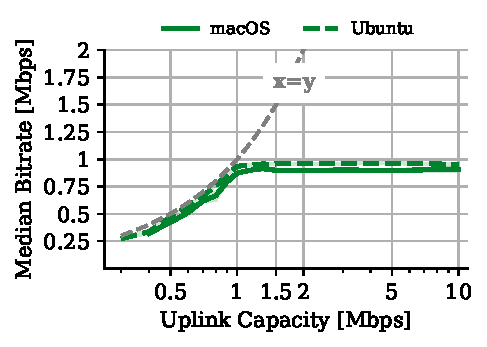
\includegraphics[width=\textwidth,keepaspectratio]{figures/static_mac/uplink_Meet_comparison.pdf}
    \caption{Meet}
	\label{subfig:uplink_meet_bitrate_mac}
\end{subfigure}\hfill
\begin{subfigure}[t]{0.4\textwidth}
    \centering
    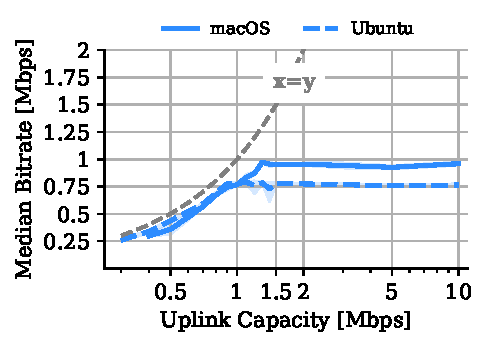
\includegraphics[width=\textwidth,keepaspectratio]{figures/static_mac/uplink_Zoom_comparison.pdf}
    \caption{Zoom}
	\label{subfig:uplink_zoom_bitrate_mac}
\end{subfigure}\hfill
\begin{subfigure}[t]{0.4\textwidth}
    \centering
    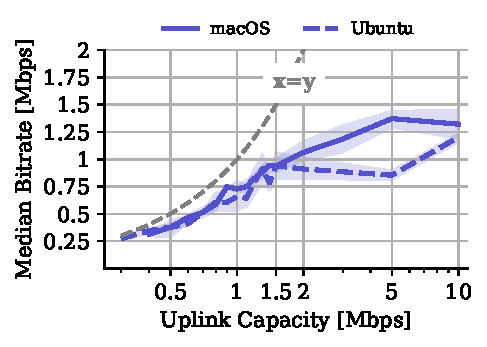
\includegraphics[width=\textwidth,keepaspectratio]{figures/static_mac/uplink_Teams-Chrome_comparison.pdf}
    \caption{\teamsbrowser}
	\label{subfig:uplink_teams_chrome_bitrate_mac}
\end{subfigure}\hfill
\caption{Comparison of uplink network utilization between macOS and Ubuntu under different shaping levels. The bands represent 90\% confidence intervals.}
\label{fig:uplink_static_mac}
\end{figure}


\begin{figure*}[t]
        \begin{subfigure}[t]{0.33\textwidth}
    		\centering
        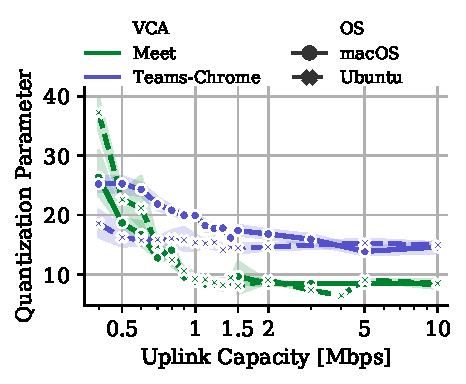
\includegraphics[width=\textwidth,keepaspectratio]{figures/static_mac/uplink_s_qpsum_comparison.pdf}
        \caption{Uplink - Quantization parameter.}
 		\label{subfig:uplink_video_qp_mac}
    \end{subfigure}%
    \hfill
	\begin{subfigure}[t]{0.33\textwidth}
        \centering
        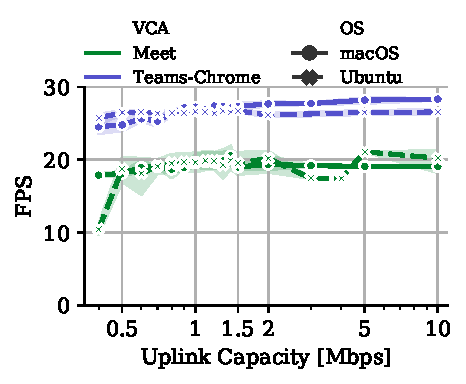
\includegraphics[width=\textwidth]{figures/static_mac/uplink_sent_framesPerSecond_comparison.pdf}
    \caption{Uplink - Frames per second.}
    \label{subfig:uplink_frames_per_second_mac}
    \end{subfigure}% 
    \hfill
	\begin{subfigure}[t]{0.33\textwidth}   
        \centering
        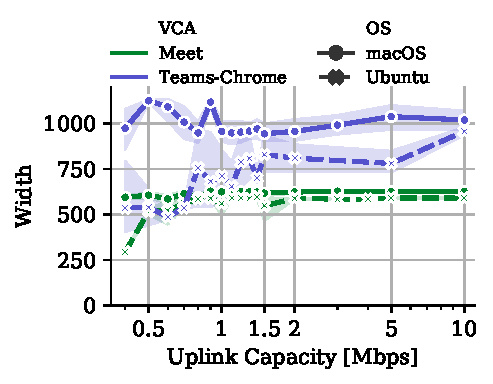
\includegraphics[width=\textwidth]{figures/static_mac/uplink_sent_frameWidth_comparison.pdf}
    \caption{Uplink - Frame width.}
    \label{subfig:uplink_frame_width_mac}
    \end{subfigure}
	\caption{Comparison of video encoding parameters between macOS and Ubuntu with 90\% confidence intervals under upstream throughput constraints.}
    \vspace{-1em}
	\label{fig:video_qual_comparison}
\end{figure*}




\begin{comment}
\begin{subfigure}[t]{0.4\textwidth}
    \centering
    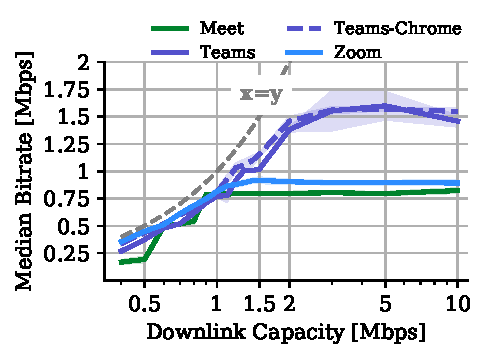
\includegraphics[width=\textwidth,keepaspectratio]{figures/static_mac/downlink_mac.pdf}
    \caption{Downlink bandwidth vs network bitrate}
	\label{subfig:downlink_bitrate_mac}
\end{subfigure}
\end{comment}

\begin{comment}
\begin{subfigure}[t]{0.33\textwidth}
		\centering
    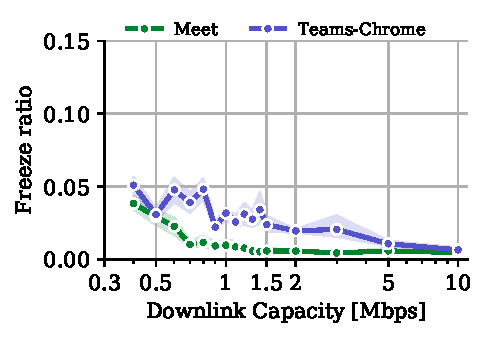
\includegraphics[width=\textwidth,keepaspectratio]{figures/static_mac/downlink_freezeRatio_mac.pdf}
    \caption{Downlink - Freeze Ratio}
 	\label{subfig:downlink_video_qp_mac}
\end{subfigure}%
\hfill
\begin{subfigure}[t]{0.33\textwidth}
    \centering
    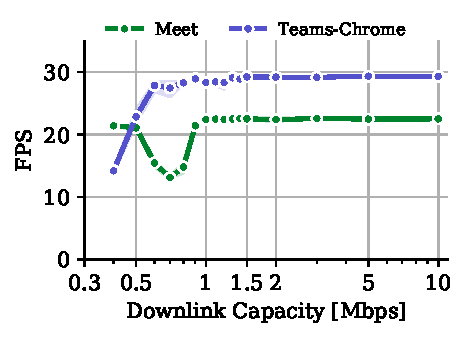
\includegraphics[width=\textwidth]{static_mac/downlink_received_framesPerSecond_mac.pdf}
\caption{Downlink - Frames per second.}
\label{subfig:downlink_frames_per_second_mac}
\end{subfigure}% 
\hfill
\begin{subfigure}[t]{0.33\textwidth}
    \centering
    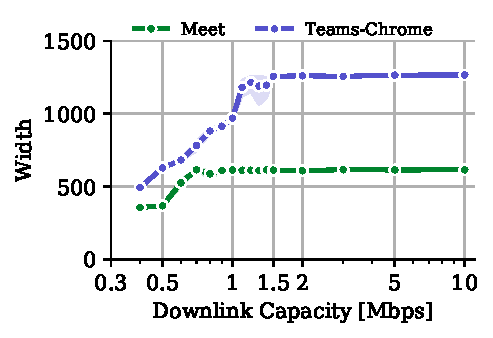
\includegraphics[width=\textwidth]{static_mac/downlink_received_frameWidth_mac.pdf}
\caption{Downlink - Frame width.}
\label{subfig:downlink_frame_width_mac}
\end{subfigure}
\newline
\end{comment}